\subsection*{7. Codificación de Fuente}

\noindent \textbf{7.1) Fundamentos de Codificación:}\par
\bigskip

\noindent a)Explique la diferencia entre codificación de fuente y codificación de canal.\par
\bigskip

\noindent La codificación de fuente se enfoca en la compresión de datos, eliminando redundancia para optimizar el almacenamiento y ancho de banda, mientras que la codificación de canal se centra en la protección de la información, añadiendo redundancia para detectar y corregir errores introducidos por el canal de comunicación. La primera reduce la información, la segunda la aumenta con un propósito protector.
\bigskip

\noindent b) ¿Qué establece el Teorema de Codificación de Fuente de Shannon?. \par
\bigskip
\noindent El Teorema de Codificación de Fuente de Shannon establece que la longitud mínima promedio de una secuencia de código para representar una fuente de información es la entropía de la fuente, dividida entre el tamaño del alfabeto de destino (generalmente bits). Es decir, permite comprimir datos hasta un límite teórico fundamental, que es la cantidad de información que realmente contiene la fuente, eliminando la redundancia. 
\bigskip

\noindent c) Defina eficiencia y redundancia de un código.\par
\bigskip

La eficiencia de un código se refiere a la relación entre la cantidad de información útil transmitida y la longitud total del mensaje codificado. Por otro lado, la redundancia de un código es la cantidad de información adicional añadida al mensaje original para permitir la detección y corrección de errores en la transmisión de datos. 
\bigskip
%---------------------------------------------------------------------------------
\bigskip

\noindent \textbf{7.2) Códigos de Longitud Variable:}
\bigskip

\noindent a) Enuncie las propiedades de un código únicamente decodificable. \par
\bigskip

Las propiedades de un código únicamente decodificable son las siguientes:
\begin{itemize}
\item 1. No puede haber ninguna palabra de código que sea prefijo de otra palabra de código.
\item 2. Cada palabra de código puede ser decodificada de manera única independientemente de las demás palabras de código.
\item 3. El proceso de decodificación es determinista, es decir, no lleva a ambigüedades o múltiples interpretaciones.
\end{itemize}
\bigskip
Estas propiedades garantizan que el proceso de decodificación sea eficiente y sin errores, permitiendo una correcta recuperación de la información transmitida a través del código.
\bigskip

\noindent b) ¿Qué es la desigualdad de Kraft? ¿Cuál es su importancia?. \par
\bigskip

La Desigualdad de Kraft es una condición que debe cumplir cualquier código de prefijo (y por extensión, únicamente decodificable). Establece que:
    \[
\sum_{i=1}^{M} 2^{-l_i} \leq 1
\]

donde l\_i son las longitudes de los códigos. Si se cumple, existe un código de prefijo; si no, es imposible construirlo.

\bigskip
\noindent c) Explique el algoritmo de Huffman paso a paso. \par
\bigskip

\noindent \textbf{Paso a Paso del Algoritmo de Huffman}
\begin{enumerate}
    \item \textbf{Paso 1}: Listar todos los símbolos con sus probabilidades (de mayor a menor) 
    \item \textbf{Paso 2}: Tomar los dos símbolos con menor probabilidad y combinarlos en un nuevo nodo (sumar sus probabilidades)
    \item \textbf{Paso 3}:Volver a ordenar todos los nodos (símbolos y combinados) por probabilidad.
    \item \textbf{Paso 4}: Combinar los dos menores nuevamente y reordenar hasta que quede un solo nodo.
    \item \textbf{Paso 5}: Recorrer cada rama y formar el código único para cada símbolo.
    
    
\end{enumerate}







%---------------------------------------------------------------------------------
\bigskip

\noindent \textbf{7.3)} Para el alfabeto (A, B, C, D, E) con probabilidades (0.1, 0.2, 0.15, 0.4, 0.15):\par

\noindent a)Calcule la entropía de la fuente. \par
\bigskip
\noindent \begin{equation*}
H(X) = \ 0.1 \log_2 (1/0.1) + 0.2 \log_2 (1/0.2) + 0.15 \log_2 (1/0.15) + 0.4 \log_2 (1/0.4) + 0.15 \log_2 (1/0.15) = 2.146 \text{ bits/símbolo}
\end{equation*}



\noindent b) Diseñe un código de Huffman. \par

\begin{figure}[H]
    \centering
    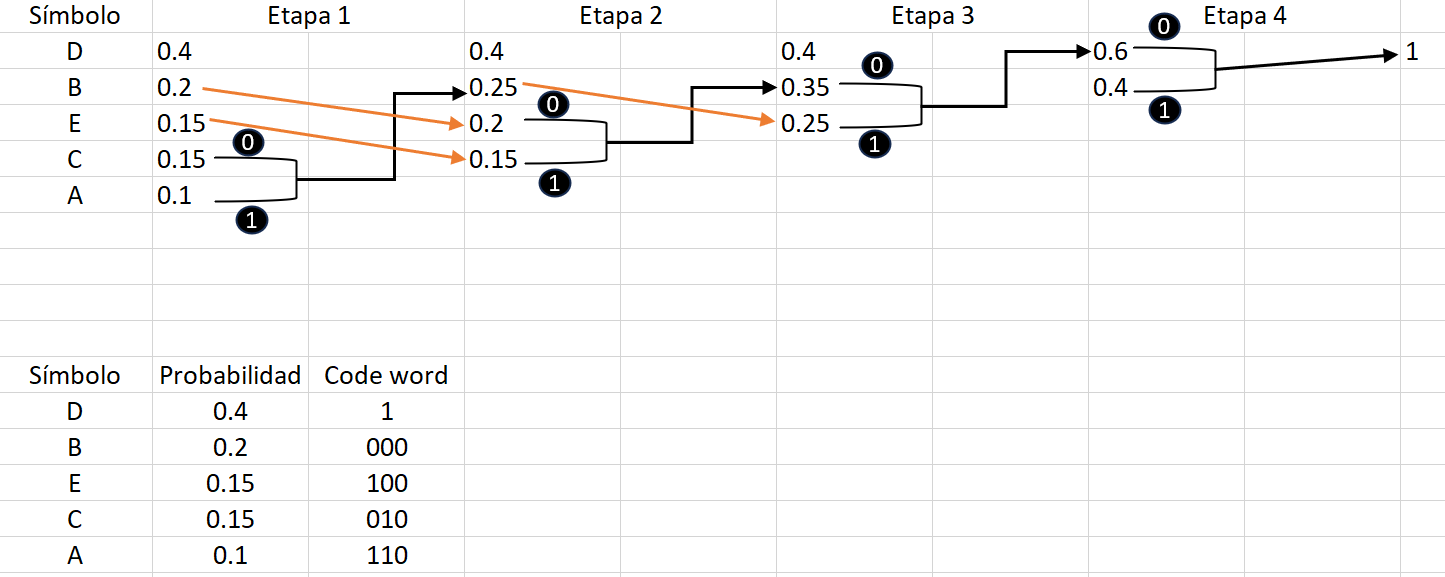
\includegraphics[width=0.8\linewidth]{Captura de pantalla 2025-09-08 164244.png}
    \caption{Diagrama de Huffman}
    \label{fig:placeholder}
\end{figure}

\noindent c) Calcule la longitud media del código. \par
\bigskip
\noindent \begin{equation*}
L = \sum_{i=1}^{n} p_i l_i= \\(0.4 \times 1) + (0.2 \times 3) + (0.15 \times 3) + (0.15 \times 3) + (0.1 \times 3) \\
= 0.4 + 0.6 + 0.45 + 0.45 + 0.3 = 2.2 \text{ bits/símbolo}
\end{equation*}

\noindent d) Calcule la eficiencia del código. \par

\begin{align*}
\eta &= \frac{H(X)}{L} \times 100\% \\
\eta &= \frac{2.146}{2.22} \times 100\% = 97.54\%
\end{align*}
